\documentclass[12pt, a4paper]{report}

\usepackage{listings, graphicx, geometry, etoolbox, parskip, caption, subcaption, hyperref, lmodern, minted}
\usepackage{listings}
\usepackage{xcolor}
\usepackage[section]{placeins}
\usepackage[utf8]{inputenc}
\usepackage[T1]{fontenc}
\usepackage{pdfpages}
\lstset { %
    language = C++,
    backgroundcolor=\color{black!5}, % set backgroundcolor
    basicstyle=\footnotesize,% basic font setting
}
\definecolor{LightGray}{gray}{0.9}
\definecolor{Arsenic}{rgb}{0.1, 0.1, 0.1}
%=================================================================
\makeatletter
% \patchcmd{<cmd>}{<search>}{<replace>}{<success>}{<failure>}
% --- Patch \chapter
\patchcmd{\@makechapterhead}{50\p@}{\chapheadtopskip}{}{}% Space from top of page to CHAPTER X
\patchcmd{\@makechapterhead}{20\p@}{\chapheadsep}{}{}% Space between CHAPTER X and CHAPTER TITLE
\patchcmd{\@makechapterhead}{40\p@}{\chapheadbelowskip}{}{}% Space between CHAPTER TITLE and text
% --- Patch \chapter*
\patchcmd{\@makeschapterhead}{50\p@}{\chapheadtopskip}{}{}% Space from top of page to CHAPTER TITLE
\patchcmd{\@makeschapterhead}{40\p@}{\chapheadbelowskip}{}{}% SPace between CHAPTER TITLE and text
\makeatother
% Set new lengths
\newlength{\chapheadtopskip}\setlength{\chapheadtopskip}{0pt}
\newlength{\chapheadsep}\setlength{\chapheadsep}{10pt}
\newlength{\chapheadbelowskip}\setlength{\chapheadbelowskip}{10pt}

\newgeometry{
    top=2cm,
    bottom=2cm,
    outer=1.5cm,
    inner=1.5cm,
}
%=================================================================

\title{CPS2004-Logistics}
\author{Keith Farrugia}
\date{January 2024}

\begin{document}

\maketitle
\newpage
\tableofcontents
\newpage
\includepdf[pages={1}]{Images/"CPS2004 Plagiarism Form - Keith Farrugia 11104L.pdf"}
\newpage

\chapter{Introduction}
Link to video: \\ 
\url{https://drive.google.com/file/d/1YCeyzTcugy7-0OHqYYU_CrFRl5mFCWSG/view?usp=sharing}\\
Link to Code Repository: \\
\url{https://gitlab.com/KeithFarrugia/cps2004_logistics.git}\\
\section{Basic Overview}
The following report will serve to highlight and explain the several features and design implementations which were required for the CPS2004 - Object Oriented Programming assignment. 

With regards to the report's structure, it will follow the main Tasks as listed by the requirements sheets. The code being discussed in each chapter can be found in its respective file in the online code repository in GitLab, found through the link above. In other words, "Chapter 2 - Task 1" will be related to the code that can be found in the Task 1 folder, further information about the code organization can be found in the ReadMe.md file.

\chapter{Task 1}
\section{Information about Task 1}
Since the code structure is mirrored almost completely in both Java and C++, the explanations will be mostly general without going into the minute details. When there is a significant difference in the implementation of either language's program, this will be mentioned.

\section{UML Diagram}
\begin{figure}[!htp]
  \centering
    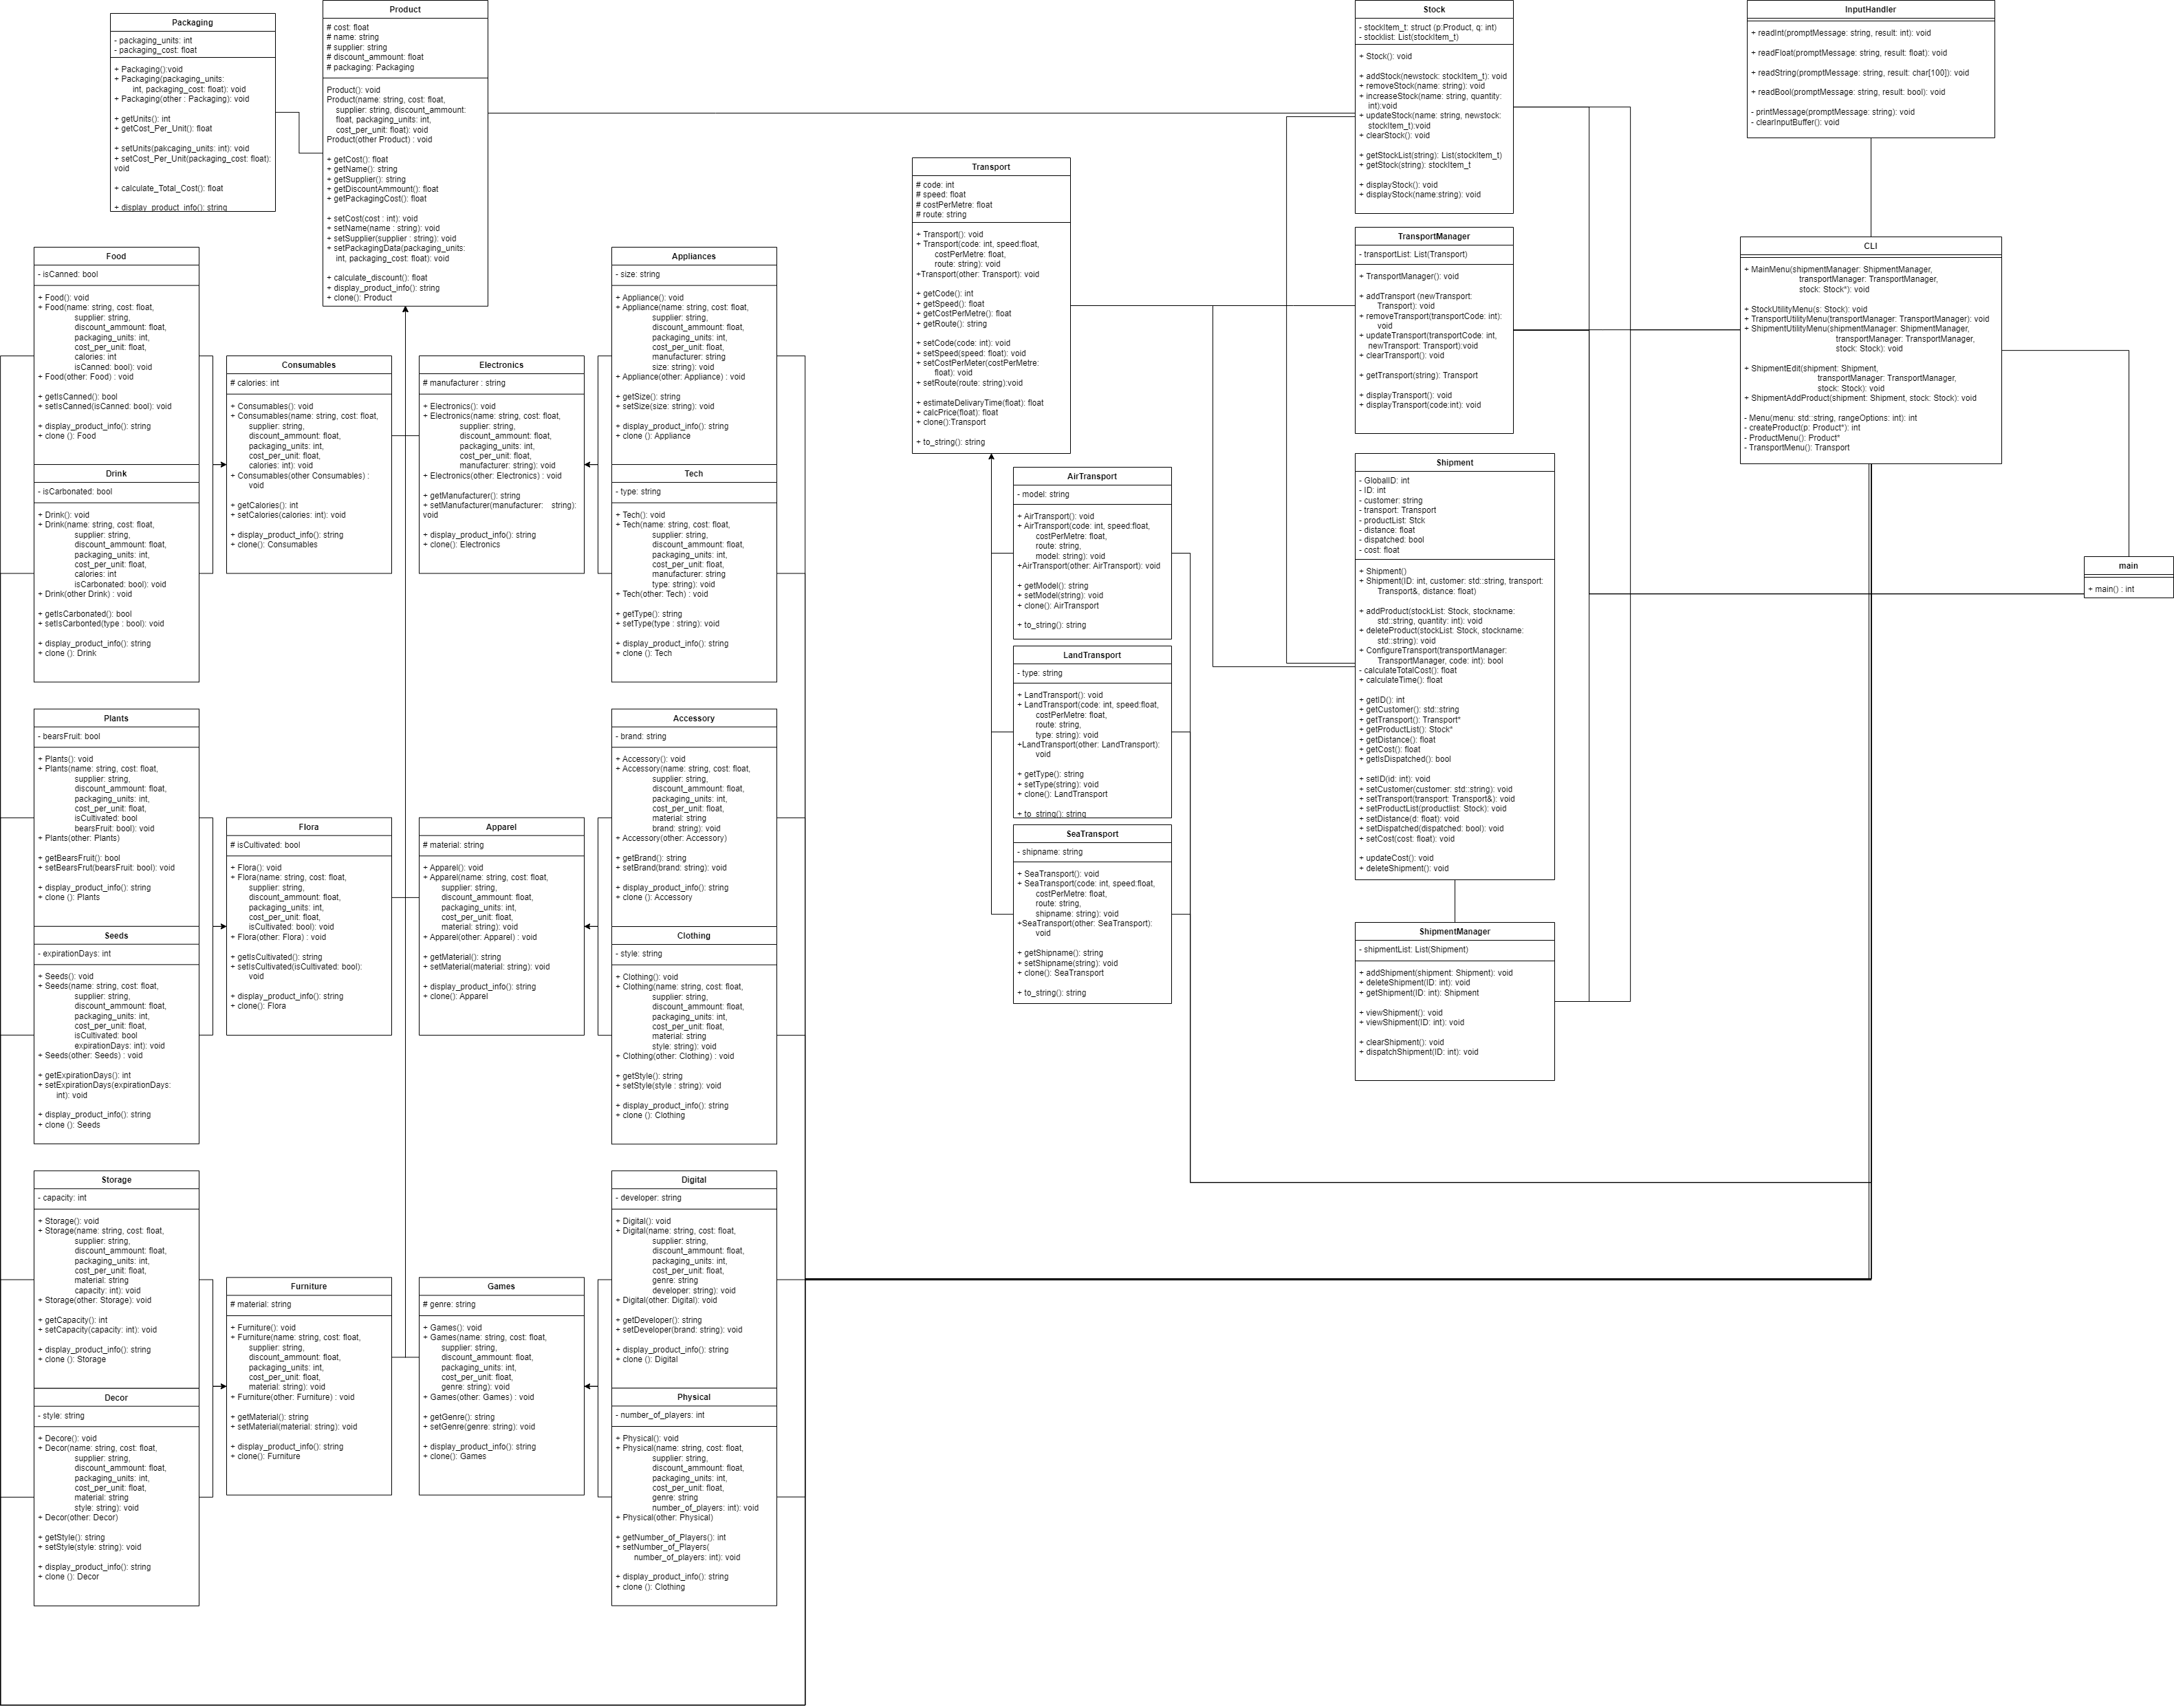
\includegraphics[width=15cm]{Images/OOP UML Diagram.drawio.png}
    \caption{UML Diagram}
  \hfill
\end{figure}

\section{Implementation}
The following subsections will tackle the classes which make up the implementation for the first task of the assignment. Each section relates to a class or set of classes and their functions. 


\subsection{Product}
The product hierarchy is a storage hierarchy, its only purpose being to hold and organize the various variables related to the product and its subclasses. The various variables that create and differentiate the subclasses can be seen in the UML diagram (Figure 2.1). The product makes use of the packaging class to hold data related to packaging, such as the amount of packaging units and the cost per unit both of which are product-specific. In terms of functions and methods, all product classes follow a set pattern. The method list includes;
\begin{itemize}
  \item 3 Constructors:
     \begin{description}
     \item[Defualt:] A blank constructor taking no parameters.
     \item[Parameterized:] A Constructor which takes all variables relating to that product.
     \item[Copy Constructor:] A constructor which is used to create an instance which holds the same values as the instance passed as a parameter.
     \end{description}
  \item Getters and Setters per variable of each product
  \item Display product info method which returns a string which can then be printed to the terminal.
  \item A clone function which is polymorphed in the subclasses and makes use of the copy constructor to return a copy of the current instance
\end{itemize}
Another function worth noting is the "calculate\_discount" function which returns the product's discount only if the month is December and else returns 1 which is equivalent to no discount at all. This is then multiplied with the total cost calculated by some other process. The getter for packaging also returns the cost calculated by the packaging class as it was deemed that there was no use for returning the actual packaging instance.

In terms of supplier, each Product instance was required to have a supplier attached. Although the supplier could have warranted the creation of its own specific class, since there were no real constraints put upon the supplier or much functionality required relating to it, the supplier was specified as a single string which aided simplicity as well as reduced complexity for the user, as the same supplier name could be used for multiple products without needing additional validation and other functions.

The Packaging class is similarly lightweight, composed of the 2 variables previously mentioned, a similar 3 constructor set, Getters and Setters for the relative variables, and a display string function mirroring the product classes. The "calculate\_Total\_cost()" multiplies the cost and unit number, returning the result.

\subsection{Transport}
The Transport class hierarchy serves the same purpose as that of the Product hierarchy. The variables are once again listed in the UML Diagram (Figure 2.1). The overall construction of method listings also mirrors those of the product class i.e.; each Transport class includes a 3 constructor set, as well as Getters and Setters for all the respective variables. The classes also include their own clone function which serves the similar purpose of returning a copy of the current instance. The "to\_string()" method also serves the same purpose as its "display\_product\_info()" function, returning a display string. What is worth noting are the 2 new functions estimateDeliveryTime which given a distance calculates the time based on the set vehicle speed, and calcPrice which given a similar distance calculates the price based on the transport cost.

\subsection{Stock}
To organize the methods relating to stock as well as create the stock item object, the class stock was created. Its main purpose is to hold a list of products and their quantities, this is done through the stockItem object. In C++ stock item is a struct of a pointer to a product and an integer quantity, while in Java another class was created inside stock to serve as a substitute for the struct. Stock is only implemented with a default non-parameterized constructor, since upon creation, it should hold an empty list. In terms of functions, Stock is equipped with the following:\\

\begin{description}
   \item [addStock():] Takes a stockItem object which is added to the current stock, but only if another item in stock does not already use the name.
   \item[removeStock():] Takes a string for the stock's name, searches for it and then deletes it from the list 
   \item[updateStock():] Takes the name of the stock to update and a newstock which serves as the updated version. If the name corresponds with one of the stocks in the list, the function then makes sure that the new updated stock does not have the same name as another stock in the list or has the same name as the stock that it is meant to replace. The old stock is then removed and the new one is added.
   \item[increaseStock():] Takes the name of a stock and a quantity, and adds the quantity to that of the corresponding stock in the list, effectively creating a way to order more stock of that item.
   \item[clearStock():] This clears the current list of stock items. Its importance is more visible in C++ due to memory management since Java has the garbage collector. 
   \item[getStock():] Takes the name of a stock and returns a reference to the object if it exists in the list.
   \item[displayStock():] This function is overloaded, having two versions. If a string is provided it only prints the data relating to the stock corresponding to that name. If nothing is provided then the function displays all stock in the list.
\end{description}

\subsection{Transport Manager}
Similarly to stock, this class is used to organize all the functions relating to the list of saved transport methods, as well as holding the list itself. The functions provided are the following:\\

\begin{description}
   \item [addTransport():] Takes a Transport object which is added to the current transport list, but only if another item in the transport list does not already use the code.
   \item[removeTransport():] Takes a transport code, searches for it and then deletes it from the list 
   \item[updateTransport():] Takes the code of the transport to update and a newTransport which serves as the updated version. If the code corresponds with one of the Transport in the list, the function then makes sure that the newly updated transport does not have the same code as another Transport in the list or has the same code as the Transport that it is meant to replace. The old transport is then removed and the new one is added.
   \item[clearTransport():] This clears the current list of transports. Again its importance is more visible in C++ due to memory management since Java has the garbage collector. 
   \item[getTransport():] Takes the code of a transport and returns a reference to the object if it exists in the list.
   \item[displayTransport():]This function is overloaded, having two versions. If a code is provided it only prints the data relating to the transport corresponding to that code. If nothing is provided then the function displays all transports in the list.
\end{description}

\subsection{Shipment}
The Shipment class takes care of a client's order. It makes use of both the Transport Class hierarchy to hold a single transportation method, and the stock class to hold a list of stocks which the user wants to buy. Shipments are given IDs which are generated automatically using a static GlobalID which in turn is incremented every shipment. Two important variables are the dispatched variable which makes sure a shipment is not updated once it has been dispatched, and the cost which is only updated when a shipment is edited. Apart from the relative Getters and Setters, Shipment also provides the following functions:

\begin{description}
   \item [addProduct():] This takes the stocklist from which it is to find the requested product, the product name, and the quantity of the ordered product. The function searches for a product in the stocklist, and if it is found copies its data into the stocklist for the shipment. This way if the product in the stocklist is changed, the product in the shipment is kept the same. No product is added if the shipment is dispatched.
   \item[deleteProduct():] Takes the name of the product to delete and deletes it through the relevant stock function. No product is deleted if the shipment is dispatched.
   \item[ConfigureTransport():] Similarly to addProduct, this function takes the list from which the transport should be copied and the transport's code. Transport cannot be configured if shipment is dispatched.
   \item[calculateTotalCost():] This calculates the cost making use of the respective transport and stock functions. 
   \item[calcualteTime():] This calculates the time using the relative transport function
   \item[updateCost():] This updates the cost variable using the calculateTotalCost() function. Cost cannot be updated if the shipment is dispatched.
   \item[deleteShipment():] This deletes the shipment clearing the related objects as well. This is more important for freeing resources hence dispatched is not checked.
\end{description}

A Note on the shipment class: Similarly to the supplier mentioned in Product, Customer could have warranted its own class but again since no functionality relating to customer was required, the simpler alternative of a string was implemented.

\subsection{ShipmentManager}
ShipmentManager serves a similar process to TransportManager, where it holds the functions relating to a list of shipments and then the shipment list itself. It provides the following functions:
\begin{description}
   \item [addShipment():] Takes a shipment object adding it to the list, if and only if its ID is not already in use.
   \item[deleteShipment():] Takes a shipment ID and removes it from the list after checking if it has been dispatched.
   \item[vewShipment():] This function is again overloaded, one function prints the whole list while the other a specified instance. 
   \item[clearShipment():] Clears the shipment list from all shipments. It does not check if shipments have been dispatched as it is important to allow the user to have some way to start from scratch/ clear the current list.
   \item[dispatchShipment():] Dispatches a shipment making it unable to be edited.
\end{description}

\subsection{InputHandler}
This class serves the simple function of displaying the prompts and taking the correct input depending on the function, raising an exception if the input is incorrect.

\subsection{CLI}
As required the CLI class handles console interaction, mostly relating to menus user input and combining the previously discussed classes into one cohesive process. The more utilitarian functions are the following.

\begin{description}
   \item [createProduct():] This function is used to reuse the related function calls used in the creation of the Parent Product Class. Since all subclasses require the creation and user input to these variables, instead of repeating the input, the function was created to minimise the code length. 
   
   \item [Menu():] This is the basic menu function that given a string holding the menu to be displayed makes sure that the user input falls within the specified range before returning it.  
   
   \item [ProductMenu():] This function displays to the user the 12 subclasses from which he/she can choose from which to create the product. Through the use of a switch, the function then creates the product and asks the user to fill in the relative variables. In both language implementations, there is heavy use of exceptions to both recognise when the user's input is not what was expected and when the object creation has failed. In C++ unique pointers are used to make sure that the object is deleted from memory in the case that an exception is raised. It returns the created Product.
   
   \item [TransportMenu():] This serves a similar purpose to Product. It displays a menu of the 3 different transport classes and depending on what the user chooses, the function takes the input related to that class, returning the created Transport.
   
   \item[ShipmentAddProduct():] This function is used to add products to the shipment. The user is presented with a menu to decide whether to stop adding Products or adding another one. If the user wants to add a Product then the product name and quantity are asked and the product name quantity and the list of stock are sent to the shipment class to be used by the addProduct method.
   
   \item[ShipmentEdit():] This function is used to edit a shipment. The functionality is relatively basic, editing includes adding a product which calls the ShipmentAddProduct() function, removing a product which deletes a product whose name is input, and changing the configured Transport, where the transport code is inputted, and the ConfigureTransport() function is called. If this function were to fail, the transport would be rolled back to the previously set transport.
\end{description}

The following functions are less dependent on others and are the Main menus for each major component.
\\

\begin{description}
   \item [StockUtilityMenu():] This Is the function which allows the user to access the various parts relating to stock. It presents 8 options to the user. Adding a product simply makes use of the ProductMenu() function to create the product, ask for the quantity, and add it to the stock list. Deleting a product asks the user for the product's name and calls the stock removeStock() function. Updating the product is a somewhat simplistic implementation where upon receiving the name of the product to update, the user is then asked to input a complete product through the ProductMenu() function which then is used to replace the chosen product in the updateStock() function. This method was chosen since the implementation is simpler than having a separate menu for each product subclass to allow the user to change variables separately. Increasing the stock asks the user for the name of a product and the quantity to increase the stock buy, the related stock function is then called. Relating to printing there are two options one which asks the user for the specific product to print while the other prints all the stock. Delete Stock clears the stock list using the related function. The last option is to quit the menu.
   
   \item [TransportUtilityMenu():] The transport utility menu follows the same structure as its stock counterpart. Add Transport uses the TransportMenu() function to create a transport and adds it to the list inside transportManager, Delete Transport asks the user for a code and makes use of that code through the removeTransport() function to delete the relative transport. Update Transport takes a similar approach to the stock menu where a new transport object is created and after the user inputs the code of the transport to be updated, the transport is replaced. Printing again provides 2 options to to user, either to print all transports in the list or to print a specific transport based on the inputted code. The final 2 options are to clear the transport through the clearTransport() function in TransportManager and the option to quit the menu.
   
   \item [ShipmentUtilityMenu():] The Shipment menu similarly provides 8 options. Add Shipment asks the user to input the basic variables first. For Transport, the user is asked to input a code and the transport is then found from the TransportManager's list. to add products the ShipmentAddProduct() function is called. When a shipment is added to the list the shipment's ID is printed to the user. Deleting a shipment involves the user inputting the relative ID and the function then calls the deletShipment function. For editing the function first asks for the ID and checks that there exists a shipment related to it, and then calls the ShipmentEdit() function. Dispatching a shipment asks the user for the shipment's ID and then calls the dispatch function. Similarly to before, printing a shipment allows the user to choose whether to print the entire shipment list or just a single shipment which takes a shipment's ID. Clearing shipments calls the clearShipment() function and finally, the last option is for the user to quit the menu.
   
   \item [MainMenu():] The MainMenu() is a simple 4 option menu which allows the user to navigate to the aforementioned 3 menus for the different components, or to exit the program.
\end{description}

It is worth noting that the CLI class does not provide the user with the option of saving and loading data as these functions will be implemented in the later Tasks.

\subsection{Main}
The main function doesn't offer much in terms of code and simply serves the function of holding the instances for Stock, ShipmentManager and TransportManager and calls the MainMenu in CLI.

\chapter{Task 2}
The code base which is being refactored is that which was written in Java. The relevant code can be found in the Task 2 file in the online repository.

\section{UML Diagram}
\begin{figure}[!htp]
  \centering
    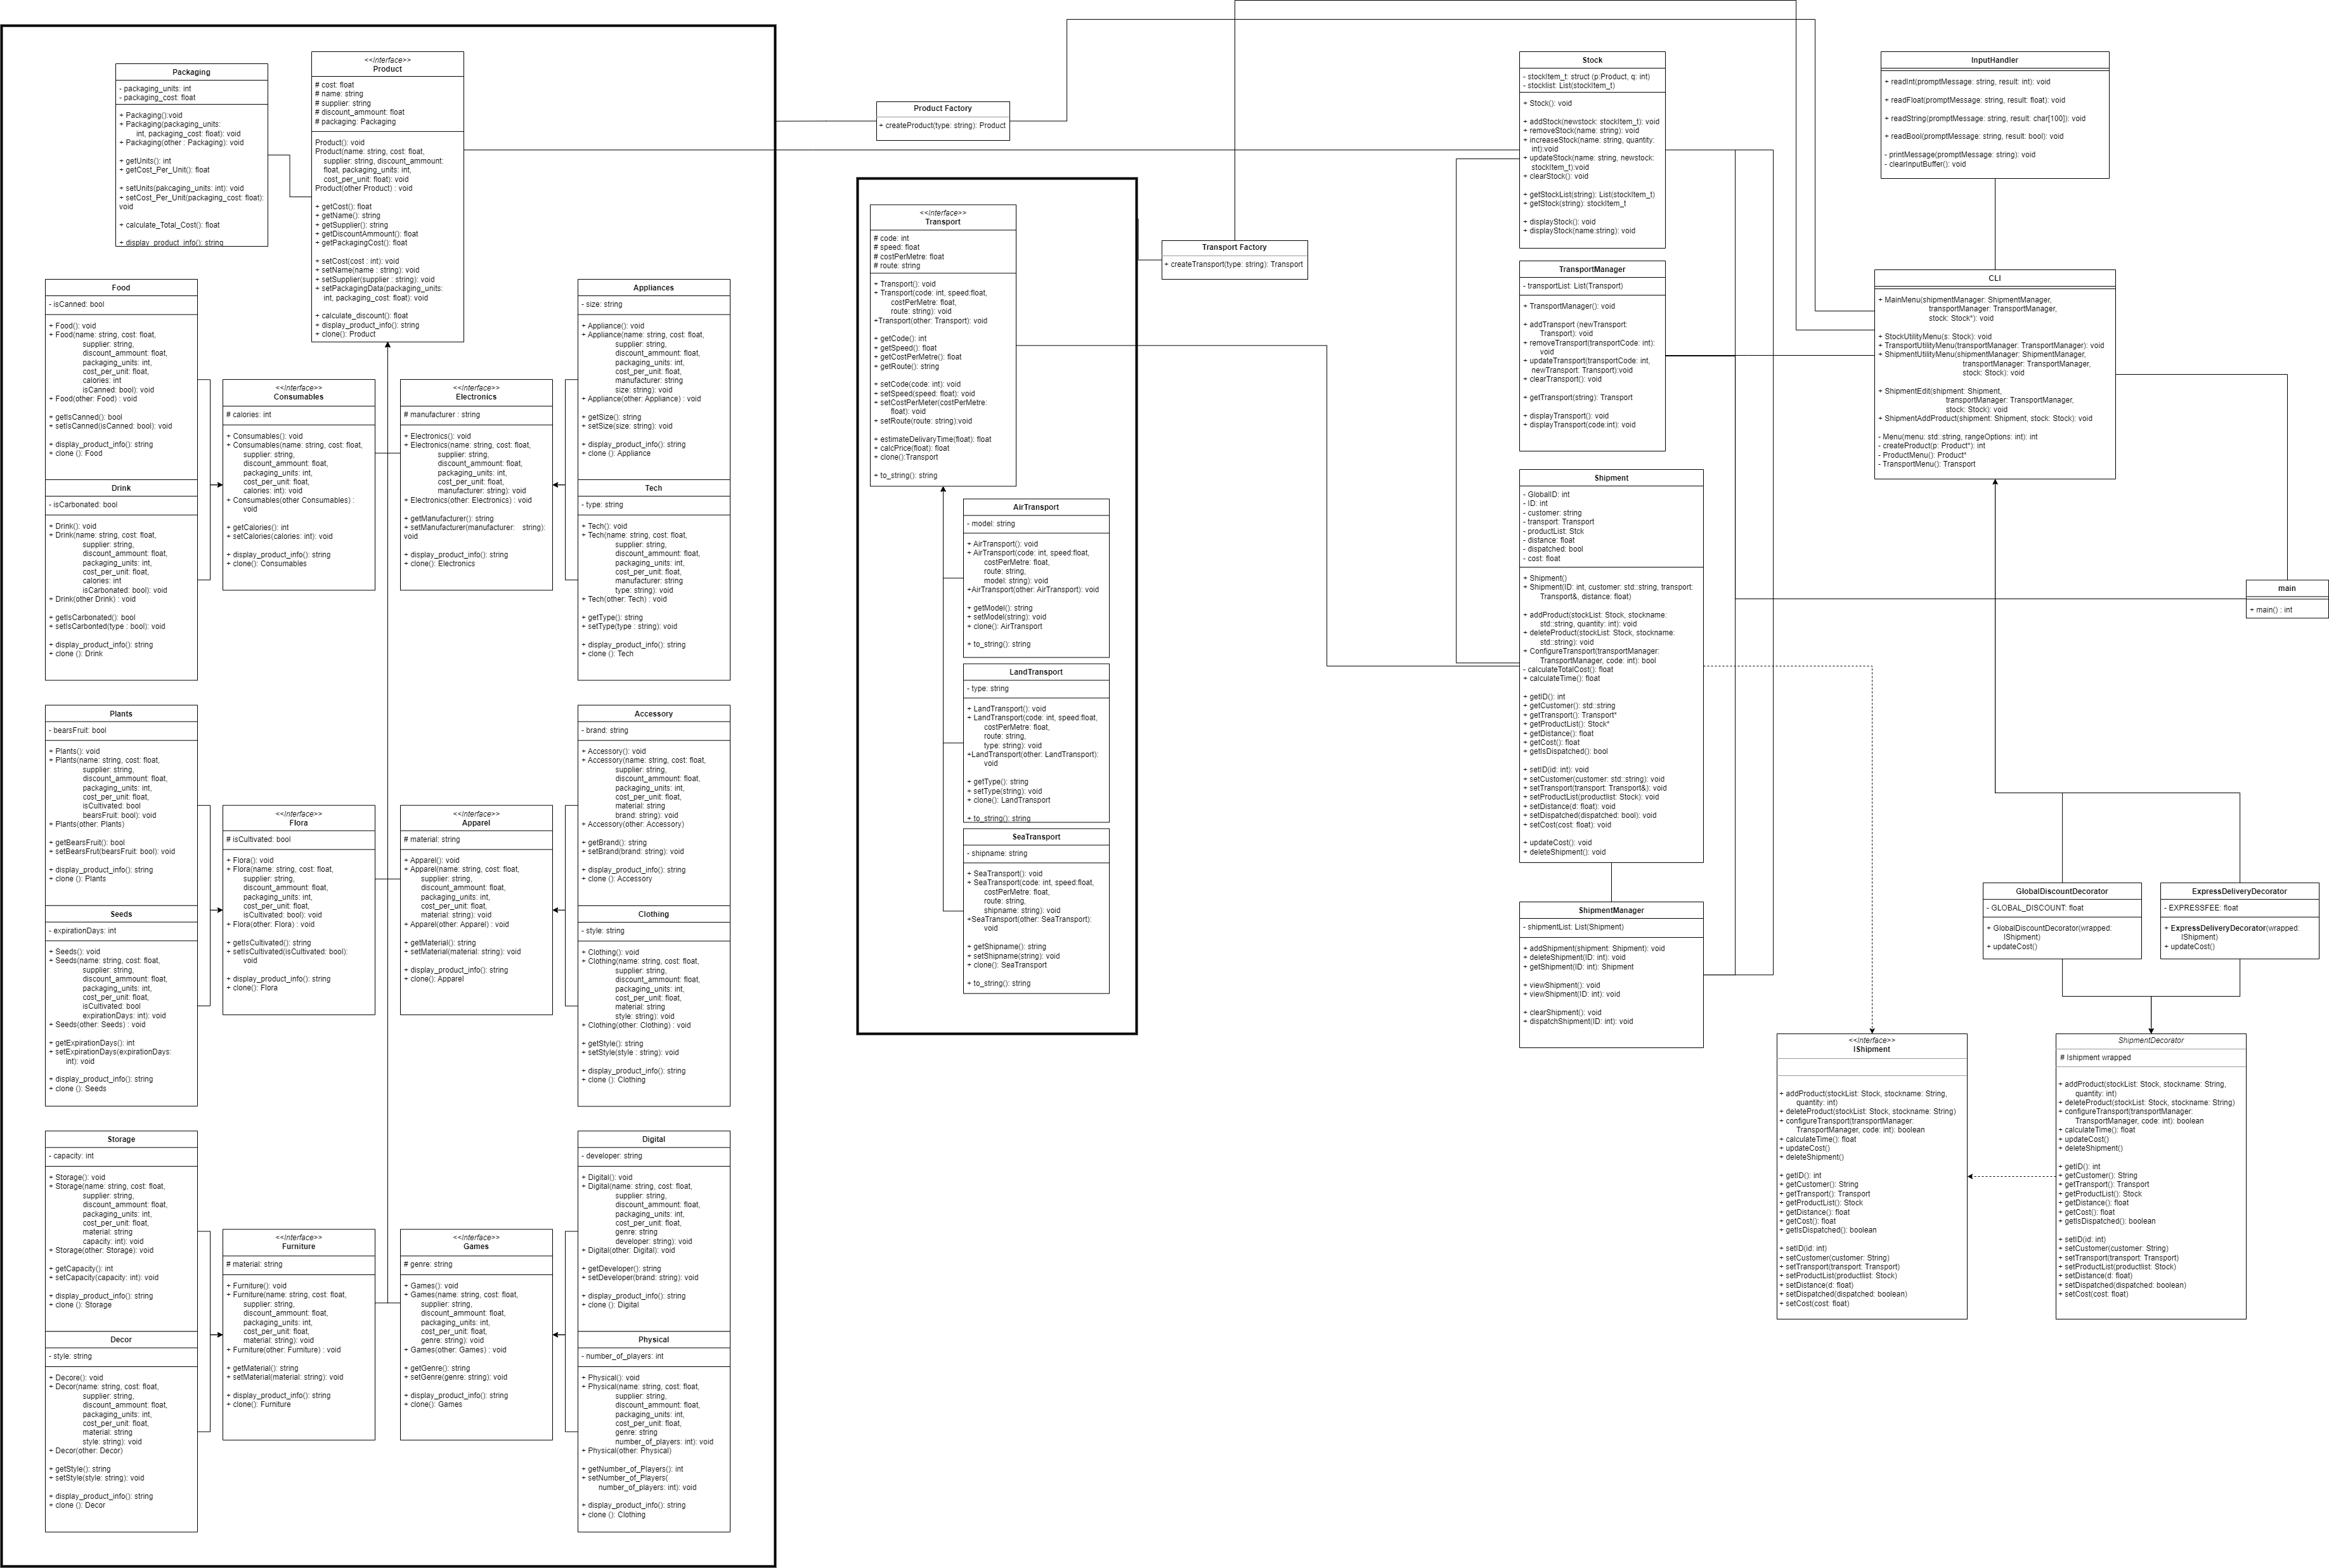
\includegraphics[width=15cm]{Images/OOP UML Diagram 2.drawio.png}
    \caption{UML Diagram}
  \hfill
\end{figure}

\section{Factory Pattern}
The Factory pattern has only affected the Product and Transport hierarchy, therefore only these will be discussed in the following section.

The first step in conversion to the factory pattern is to transfer the current hierarchy to make use of interfaces instead of the inheritance-based approach taken in Task 1. This meant that all parent classes of both hierarchies were now abstract and so although functions were stated in the parent classes the bodies had to be implemented in the subclasses. Variables were also to be shifted down to the base concrete classes. 

The Factory Class is almost identical in function for both hierarchies where given a string containing the type, the respective subclass would be created and returned to the calling function. This change in implementation only really affected the ProductMenu and TransportMenu functions in CLI which now made use of the factory in order to create the objects. An issue that arose was the actual setting of the variables inside the objects created by the factory class. Since the Factory Pattern's purpose is to aid in object creation, user input is not usually accepted in the factory creation function. So in order to fill the variables of the intended object with the user's intended input there were 2 approaches. 

The first was to pass additional variables to the string holding the type in the factory creation function, which would then be used to fill the values in the respective object. This approach was not taken since each time a subclass would be added, which would require an additional parameterized variable, hence increasing the number of parameters the factory method would require, all function calls to the factory method from external classes would need to be updated to accommodate the increase in parameters. This would invalidate one of Factory Pattern's intended purposes which is to provide an interface which is easy to extend.

So in order to make better use of the Factory Pattern, the ProductMenu() and TransportMenu() functions acted as sort of rapper functions. Since they already served a similar function to the factory pattern and still required information on the class hierarchy to provide the required input to the user, these methods now make use of the Factory Pattern for object creation but still, the type cast the object to access the relative getters and setters so that the variables can be set. This hence made use of the Factory Pattern to aid in object creation and still allowed for easy extendability where if a subclass were to be added only an if statement in the factory function would need to be added and a switch case in the respective menu function.

\section{Decorator Pattern}
The Decorator Pattern was much smoother to incorporate not requiring any change to the old code. The Shipment class was kept mostly the same except this time it implemented the IShipment interfaces which listed all the functions available in the shipment class. The ShipmentDecorator also implemented the same interface and was abstract. In order to fulfil the purpose of the decorator pattern and serve as a wrapper for the class, the ShipmentDecorator also holds an instance of an object that implements the IShipment interface. Being the parent class ShipmentDecorator also sets the default implementation for the functions specified in the interface where it simply calls the instance's function respectively.

There are 2 concrete Decorators which have been implemented. EpressDeliveryDecorator which overloads the updateCost function to add a 30\% cost increase to the shipment cost as if it were the increased cost for express delivery. The Second decorator is the GlobalDiscount which also overrides the updateCost() function this time to decrease 20\% from the shipment's cost. 

To make use of these 2 Decorators, two other options were added to the CLI ShipmentUtilityMenu where one makes use of the GloablDiscount as a sort of coupon activation that reduces 20\% while the other option simply states to activate an Express Delivery. Both Functions first ask the user to input the shipment's ID and then pass the found instance to the classes depending on the option, after which the updateCost() function is called.

\section{Comments on the Design Pattern's Effects}
The Factory Pattern served to decouple the object creation from most of the rest of the codebase. The changes made to both hierarchies also aided in decoupling the parent class from the child classes to some extent allowing for easier expansion later on. The Decorator Pattern also aided in adding additional functionality without needing to change the base function. Shipments could both add the cost of express shipping as well as a coupon discount without needing to typecast the object and recast it.

\chapter{Task 3}
Since most of the following code relating to the Task 3 implementation is repetitive, most of the explanation is generalised in order to avoid restating the same concepts. This Task continues to build on the Java version of the code base more specifically the Task 2 implementation.

\section{PBLogistics.proto}
The Protobuf file can be found in the Serialization folder. It uses messages to closely mimic the hierarchal structures of Transport and Stock as well as the shipment class. Since protocol buffers don't make use of inheritance, parent classes are decoupled and referenced through an instance in the child class. When multiple subclasses are combined such as with the PBStockItem, the oneof structure is used. All lists of classes such as the ones in stock (list of products), transport manager (list of transports) and shipment manager (list of shipments), were also mirrored inside the .proto file to simplify serialization.

\section{Java Integration}
In order to integrate the use of protocol buffers for serialization, 2 new methods were created in the classes that required serialization. These were the copyFromProto and copyToProto functions. Their purpose was to convert to and from the proto-generated objects facilitating the process. Since the lists of hierarchies for both products and transport were of the parent class type it was important to implement these functions in order to be polymorphed and overridden so that the subclasses were able to store their values. The copyToProto() function usually took a builder of the protobuf object for which the class should copy a version of the values it currently holds. The copyFromProto took an object of the required protobuf type and filled the current java object instance with a copy of the variables stored in the protobuf object. When it came to lists of objects which formed part of a hierarchy such as with stock and transportList, the implementation for conversion was slightly more complicated. The copyToProto function would take an object which in the .proto file was specified as repeated. The addAll function would then be called and the stream().map() function from Lists is then used to traverse the list creating protobuf objects which are set through the hierarchie's respective copyToProto() function. When copying from a protobuf list, in order to check which subclass was to be created the function makes use of the has* function which was created due to the typeof key keyword inside the .protofile. This allows the program to then create a class of that subtype and push it to the list. It is here that the factory pattern is used more effectively since the function does not require the knowledge of the class hierarchy. 

The Serialize.java holds the facades for loading and saving. Both functions load/save the 3 main data structures (Stock, TransportManager, ShipmentManager) hence needing them as parameters. The save function creates the builder equivalent for all 3 structures filling each one with the respective copyToProto call. After the builders are built the data is serialized and written to its respective file. The load function parses the files filling the 3 data structures with the respective data. In order for the user to call these functions 2 options were added in the MainMenu in the CLI class, these being load and delete, where the respective function is called.

\section{Stock Viewer}
Since the refactoring was done in Java, the stock viewer was written in C++. firstly the Product hierarchy was copied from Task 1's implementation. Similarly to the Java hierarchy, the functions copyFromProto and copyToProto were added to each product class. The Stock class was also copied and the two methods were added. The main class is somewhat complicated in order to access the generated stock.pb file which holds the data needed to be read. The first part of the main function makes sure that the current directory is set for the stock.pb file to be accessed. The function then loads the data stored into the Stock class instance, after which the displayStock() function is called to print the stock data to the terminal.

\chapter{Task 4}
For this Task once again the server implementation was made in C++ since Java was chosen as the language for the main implementation.

\section{Protobuf File}
The first thing to notice is that the hierarchy is not being created inside the .proro file, meaning that not much data is being transferred over the client-server link. The structure PBProduct Item holds the data relevant to cost calculation which would be needed per product in the shipment's stocklist. The PBShipmentInfo holds the cost for the transport and the list of product information. PBCalculation holds the format for the calculation where the shipment information is passed as a parameter and the return type is of type Float. The reason that the return type is the message Float is that simple types seem to not be accepted and cause issues during the compilation of the file.

\section{Client Side}
The Client-side wrapper class can be found in the GRPC folder. The purpose of the class is, given a shipment, serialise that shipment using the protobuf created objects, only passing the needed variables, and then using the stub calling the server calculation.

The other half of the function is inside the shipment class where the calculateTotalCost() function was changed to now act as a facade for the rest of the program. The channel is created and the wrapper class previously mentioned is created and called from where the server-side function is then made use of.

\section{Server Side}
In the serverSide implementation, the most important part is the creation of the function which fulfils the requirements set in the .proto file. This is done in the CalcServerImpl class. The code which calculates the cost is a carbon copy of what used to be in the shipment class. The RunServer function was created following the reference code provided in the notes. When running the program a small delay is visible during the point at which the shipment's cost is being calculated which is the latency between sending and receiving from the server. The Server also prints the calculated cost.
\end{document}